\chapter{Type Systems and Type Inference}\label{ch:b3:type-systems}

Chapter~\ref{ch:b3:semantic-analysis} checked Moor's types with a few dozen lines of Rust and proved, for one operator, that the check keeps booleans out of additions. This chapter does it properly, for the $\lambda$-language of chapter~\ref{ch:b3:lambda-calculus}: rules that say which programs have which types, a theorem that says well-typed programs never get stuck, and an algorithm that finds the types of a program that declares none, the most general ones, which is how programmers in languages with inference can leave most types unwritten. It ends with a \omterm{def:b3:type-systems:type-system}{type system} that tracks not what a value is but how often it may be used: Rust's.

\section{Typing rules and derivations}\label{sec:b3:type-systems:rules}

\begin{definition}[Type system]\label{def:b3:type-systems:type-system}
A \emph{type system}\index{type system} is a set of rules that assigns types to the phrases of a language and rejects the programs to which it can assign none, so as to rule out a class of errors before the program runs.
\end{definition}

\begin{definition}[Typing context, judgement, rule, derivation]\label{def:b3:type-systems:judgement}
A \emph{typing context}\index{typing context} $\Gamma$ is a finite list of bindings $x : \tau$ of variables to types; a later binding of a name hides an earlier one. A \emph{typing judgement}\index{typing judgement} $\Gamma \vdash e : \tau$ asserts that in the context $\Gamma$, the expression $e$ has type $\tau$. A \emph{typing rule}\index{typing rule} derives a judgement from others, its premises. A \emph{typing derivation}\index{typing derivation} is a finite tree of rule applications whose root is the judgement it proves.
\end{definition}

The types of the $\lambda$-language are $\tau ::= \mathtt{int} \mid \mathtt{bool} \mid \tau \to \tau \mid \tau \times \tau$, the arrow associating to the right. Here are the rules for its core.
\begin{mathpar}
\inferrule{(x : \tau) \in \Gamma}{\Gamma \vdash x : \tau}\;\textsc{var}

\inferrule{\Gamma, x : \tau_1 \vdash e : \tau_2}{\Gamma \vdash \lambda x{:}\tau_1.\,e : \tau_1 \to \tau_2}\;\textsc{abs}

\inferrule{\Gamma \vdash e_1 : \tau_1 \to \tau_2 \\ \Gamma \vdash e_2 : \tau_1}{\Gamma \vdash e_1\,e_2 : \tau_2}\;\textsc{app}

\inferrule{\Gamma \vdash e_1 : \tau_1 \\ \Gamma, x : \tau_1 \vdash e_2 : \tau_2}{\Gamma \vdash \mathtt{let}\ x = e_1\ \mathtt{in}\ e_2 : \tau_2}\;\textsc{let}

\inferrule{\Gamma \vdash e_1 : \mathtt{bool} \\ \Gamma \vdash e_2 : \tau \\ \Gamma \vdash e_3 : \tau}{\Gamma \vdash \mathtt{if}\ e_1\ \mathtt{then}\ e_2\ \mathtt{else}\ e_3 : \tau}\;\textsc{if}

\inferrule{\Gamma \vdash e_1 : \mathtt{int} \\ \Gamma \vdash e_2 : \mathtt{int}}{\Gamma \vdash e_1 + e_2 : \mathtt{int}}\;\textsc{op}
\end{mathpar}
Integer and boolean constants have their obvious types; $-$ and $\times$ are typed like $+$, and $<$ and $==$ take two integers and give a boolean. Equality is restricted to integers so that every well-typed comparison computes: a comparison of two functions would be stuck.

\begin{definition}[Simply typed $\lambda$-calculus]\label{def:b3:type-systems:stlc}
The \emph{simply typed $\lambda$-calculus}\index{simply typed lambda-calculus@simply typed $\lambda$-calculus} is the $\lambda$-calculus restricted to terms that have a type under rules \textsc{var}, \textsc{abs} and \textsc{app}, with each parameter annotated by its type and a set of base types.
\end{definition}

The rules are syntax-directed: for each form of expression, exactly one rule can conclude about it, so a checker needs no search. It walks the tree, and for each node applies the one rule, which is a recursive call per premise (\cref{lst:b3:type-systems:check}). Recording the rule and the premises at each node builds the derivation itself.

\omcode{code/bachelor-3/06-type-systems/listings/check.rs}{17}{48}{The checker of the simply typed core: one arm per rule, one recursive call per premise; each node of the result is one node of the derivation.}\label{lst:b3:type-systems:check}

\omoutput{code/bachelor-3/06-type-systems/outputs/derive_demo.txt}{A \omterm{def:b3:type-systems:judgement}{typing derivation} printed with the conclusion first and the premises indented below it. Each line is a judgement, and the rule that proves it is in brackets.}\label{out:b3:type-systems:derive}

A derivation is a proof, and the checker is a proof search that never needs to backtrack. Drawn the usual way, with premises above the line, the subtree of \cref{out:b3:type-systems:derive} for the argument is the figure below.

\begin{omfigure}
\begin{mathpar}
\inferrule*[right=abs]{\inferrule*[right=op]{\inferrule*[right=var]{ }{x : \mathtt{int} \vdash x : \mathtt{int}} \\ \inferrule*{ }{x : \mathtt{int} \vdash 2 : \mathtt{int}}}{x : \mathtt{int} \vdash x \times 2 : \mathtt{int}}}{\vdash \lambda x{:}\mathtt{int}.\,x \times 2 : \mathtt{int} \to \mathtt{int}}
\end{mathpar}
\par\smallskip{\small Four judgements, the last four lines of \cref{out:b3:type-systems:derive}, as a tree. The leaves need no premise: a variable is looked up in the context, a constant has its type.}
\end{omfigure}

\section{Type safety}\label{sec:b3:type-systems:safety}

A \omterm{def:b3:type-systems:type-system}{type system} is only worth its rules if they guarantee something. The guarantee is stated against the \omterm{def:b3:lambda-calculus:semantics}{small-step semantics} of chapter~\ref{ch:b3:lambda-calculus}.

\begin{definition}[Type safety, progress, preservation]\label{def:b3:type-systems:safety}
A \omterm{def:b3:type-systems:type-system}{type system} is \emph{safe}\index{type safety} for a semantics if a well-typed closed program never reaches a stuck term. It is usually proved in two parts. \emph{Progress}\index{progress}: a closed well-typed term is a value or can take a step. \emph{Preservation}\index{preservation}: if $\vdash e : \tau$ and $e \to e'$, then $\vdash e' : \tau$. The \emph{canonical forms}\index{canonical form} of a type are the shapes of its closed values.
\end{definition}

\begin{lemma}[Canonical forms]\label{lem:b3:type-systems:canonical}
If $v$ is a value and $\vdash v : \tau$, then: if $\tau = \mathtt{int}$, $v$ is an integer; if $\tau = \mathtt{bool}$, $v$ is $\mathtt{true}$ or $\mathtt{false}$; if $\tau = \tau_1 \to \tau_2$, $v$ is an abstraction; if $\tau = \tau_1 \times \tau_2$, $v$ is a pair of values.
\end{lemma}

\begin{proof}
The values are integers, booleans, abstractions and pairs of values, and the rules give each one type form only: the constant rules give $\mathtt{int}$ or $\mathtt{bool}$, \textsc{abs} an arrow, the pair rule a product. So a value of an arrow type, say, can only be an abstraction.
\end{proof}

\begin{theorem}[Progress]\label{thm:b3:type-systems:progress}
If $\vdash e : \tau$, then $e$ is a value or there is $e'$ with $e \to e'$.
\end{theorem}

\begin{proof}
By induction on the derivation. A variable cannot be typed in the empty context, and constants and abstractions are values. Consider $e_1\,e_2$, typed by \textsc{app} with $\vdash e_1 : \tau_1 \to \tau_2$ and $\vdash e_2 : \tau_1$. By induction, $e_1$ is a value or steps; if it steps, so does $e_1\,e_2$ by the first congruence rule. Otherwise, if $e_2$ steps, $e_1\,e_2$ does by the second. Otherwise both are values, and by \omterm{def:b3:type-systems:safety}{canonical forms} $e_1$ is an abstraction $\lambda x.\,e$, so $e_1\,e_2$ is a \omterm{def:b3:lambda-calculus:beta}{redex} and steps to $e[x := e_2]$. For $\mathtt{if}$, $+$, \code{fst} and the others the argument is the same: either a part steps, or all the parts that are evaluated are values, of the types the rule demands, hence by \omterm{def:b3:type-systems:safety}{canonical forms} of the shapes the computing rule needs.
\end{proof}

\omterm{def:b3:type-systems:safety}{Preservation} needs one lemma: substituting a value of the right type for a variable keeps the type.

\begin{lemma}[Substitution]\label{lem:b3:type-systems:substitution}
If $\Gamma, x : \sigma \vdash e : \tau$ and $\vdash v : \sigma$, then $\Gamma \vdash e[x := v] : \tau$.
\end{lemma}

The proof is a short induction on the derivation of $e$'s type (exercise~\ref{exo:b3:type-systems:7}).

\begin{theorem}[Preservation]\label{thm:b3:type-systems:preservation}
If $\vdash e : \tau$ and $e \to e'$, then $\vdash e' : \tau$.
\end{theorem}

\begin{proof}
By induction on the derivation of $e \to e'$. For the $\beta$-rule, $(\lambda x.\,e_0)\,v \to e_0[x := v]$: the typing of the \omterm{def:b3:lambda-calculus:beta}{redex} ends with \textsc{app}, above which \textsc{abs} gives $x : \tau_1 \vdash e_0 : \tau$, and the argument has $\vdash v : \tau_1$; the substitution lemma gives $\vdash e_0[x := v] : \tau$. A \code{let} is the same. For $\mathtt{if}\ \mathtt{true}\ \mathtt{then}\ e_2\ \mathtt{else}\ e_3 \to e_2$, rule \textsc{if} types $e_2$ with $\tau$. For $2 + 3 \to 5$, both sides are integers. For a congruence step, such as $e_1\,e_2 \to e_1'\,e_2$, the induction hypothesis gives $e_1'$ the type of $e_1$, and \textsc{app} applies again. The case of \code{letrec} is exercise~\ref{exo:b3:type-systems:10}.
\end{proof}

\begin{corollary}\label{cor:b3:type-systems:safety}
A closed well-typed program never gets stuck: every term it reaches is a value or takes a step.
\end{corollary}

\begin{proof}
By induction on the number of steps, \omterm{def:b3:type-systems:safety}{preservation} keeps every term reached well-typed, and \omterm{def:b3:type-systems:safety}{progress} then says it is a value or steps.
\end{proof}

\begin{omfigure}
\begin{tikzpicture}[font=\small, >=Stealth,
  t/.style={draw, rounded corners=2pt, fill=omDef!6, minimum height=6mm, inner sep=3pt}]
  \foreach \i/\lab in {0/{$e_0$}, 1/{$e_1$}, 2/{$e_2$}, 3/{$\cdots$}, 4/{$v$}} {
    \node[t] (e\i) at (\i*2.6, 0) {\lab};
    \node[omThm, font=\footnotesize] (ty\i) at (\i*2.6, -0.6) {$: \tau$};
  }
  \foreach \i/\j in {0/1, 1/2, 2/3, 3/4} {
    \draw[->, thick] (e\i) -- node[above, font=\footnotesize, omMeth] {progress} (e\j);
    \draw[->, dashed, omThm] (ty\i.south east) to[bend right=30] node[below, font=\footnotesize] {preservation} (ty\j.south west);
  }
\end{tikzpicture}
\par\smallskip{\small \omterm{def:b3:type-systems:safety}{Progress} gives each well-typed term a next step unless it is a value; \omterm{def:b3:type-systems:safety}{preservation} carries the type $\tau$ to the next term. Together they rule out the one bad outcome, a term that is neither a value nor able to step. A run may still go on forever.}
\end{omfigure}

The test \code{safety_on_sample_programs} checks both properties along entire runs: at every step of five programs, the term is not stuck, and its type has not changed. Safety says nothing about loops, nor about errors the \omterm{def:b3:type-systems:type-system}{type system} does not track: a division by zero, an index out of range, are outside it, and a language either defines their result (Moor does) or turns them into checked run-time errors.

\section{Polymorphism}\label{sec:b3:type-systems:polymorphism}

In the simply typed calculus, $\lambda x{:}\mathtt{int}.\,x$ and $\lambda x{:}\mathtt{bool}.\,x$ are two functions. One would like to write the identity once.

\begin{definition}[Type variable, type scheme, parametric polymorphism]\label{def:b3:type-systems:polymorphism}
A \emph{type variable}\index{type variable} $\alpha$ stands for an unknown type; we print them \code{'a}, \code{'b}, \dots. A \emph{type scheme}\index{type scheme} $\forall \alpha_1 \dots \alpha_n.\,\tau$ is a type with some of its variables quantified: it stands for every type obtained by replacing them, its \emph{instances}. A function is \emph{parametrically polymorphic}\index{parametric polymorphism} if it has a type scheme, one code for all the instances. \emph{Let-polymorphism}\index{let-polymorphism} gives schemes to variables bound by \code{let}, and only types to variables bound by $\lambda$.
\end{definition}

So $\mathtt{let}\ \mathit{id} = \lambda x.\,x\ \mathtt{in}\ (\mathit{id}\ 1, \mathit{id}\ \mathtt{true})$ is well typed: $\mathit{id}$ gets $\forall \alpha.\,\alpha \to \alpha$, and its two uses take the instances $\mathtt{int} \to \mathtt{int}$ and $\mathtt{bool} \to \mathtt{bool}$. The same program with $\mathit{id}$ bound by a $\lambda$, $(\lambda \mathit{id}.\,(\mathit{id}\ 1, \mathit{id}\ \mathtt{true}))\,(\lambda x.\,x)$, is rejected: a parameter has one type in the whole body. Two rules express this:
\begin{mathpar}
\inferrule{(x : \forall \vec\alpha.\,\tau) \in \Gamma}{\Gamma \vdash x : \tau[\vec\alpha := \vec\tau]}\;\textsc{inst}

\inferrule{\Gamma \vdash e_1 : \tau_1 \\ \Gamma, x : \forall \vec\alpha.\,\tau_1 \vdash e_2 : \tau_2 \\ \vec\alpha \text{ not free in } \Gamma}{\Gamma \vdash \mathtt{let}\ x = e_1\ \mathtt{in}\ e_2 : \tau_2}\;\textsc{let}
\end{mathpar}
The side condition matters: a variable that also occurs in the type of something in $\Gamma$ is not free to vary, since that thing fixes it.

The restriction to \code{let} is what keeps inference decidable: a system where a $\lambda$-bound variable could be used at two types needs annotations. And it leaves some terms untypable for good. In $\lambda x.\,x\,x$, the variable $x$ is applied to itself, so its type $\tau$ must be a function type whose argument is $\tau$ itself: $\tau = \tau \to \tau'$, which no finite type solves.

\section{Unification and inference}\label{sec:b3:type-systems:inference}

\begin{recall}
A substitution maps variables to terms; a unifier of two terms is a substitution that makes them equal, and a most general unifier is one of which every other unifier is an instance. The occurs check refuses to bind a variable to a term that contains it (Year 2 volume, predicate logic).
\end{recall}

Inference turns typing into equations, and equations into a unification problem over type trees.

\begin{definition}[Type substitution, type equation]\label{def:b3:type-systems:unification}
A \emph{type substitution}\index{type substitution} maps \omterm{def:b3:type-systems:polymorphism}{type variables} to types and applies to a type by replacing each of its variables. A \emph{type equation}\index{type equation} $\tau_1 \doteq \tau_2$ asks for a type substitution $S$ with $S(\tau_1) = S(\tau_2)$.
\end{definition}

For type trees, Robinson's algorithm is short. To unify two types, apply the substitution found so far to both. If one is a variable $\alpha$, bind it to the other, unless it occurs in it; if both are the same constant, succeed; if both are arrows, or both products, unify the two pairs of children; otherwise fail. \Cref{lst:b3:type-systems:unify} keeps the substitution idempotent: when $\alpha := \tau$ is added, $\tau$ is substituted into every binding already present, so applying the substitution once is enough.

\omcode{code/bachelor-3/06-type-systems/listings/unify.rs}{36}{66}{Unification of two types, extending a substitution; \code{bind} refuses a variable that occurs in its value.}\label{lst:b3:type-systems:unify}

\begin{omfigure}
\begin{tikzpicture}[font=\small, level distance=8mm, sibling distance=13mm, >=Stealth,
  every node/.style={inner sep=1.5pt},
  v/.style={text=omThm, font=\ttfamily}]
  \begin{scope}
  \node {$\times$}
    child {node {$\to$} child {node[v] {\textquotesingle a}} child {node[v] {\textquotesingle b}}}
    child {node[v] {\textquotesingle a}};
  \end{scope}
  \node at (1.9,-0.8) {$\doteq$};
  \begin{scope}[xshift=3.8cm]
  \node {$\times$}
    child {node {$\to$} child {node {int}} child {node {bool}}}
    child {node[v] {\textquotesingle c}};
  \end{scope}
  \node[anchor=west, align=left, font=\ttfamily] at (6.0,-0.9) {\textquotesingle a := int\\ \textquotesingle b := bool\\ \textquotesingle c := int};
  \begin{scope}[xshift=9.8cm]
  \node {$\times$}
    child {node {$\to$} child {node {int}} child {node {bool}}}
    child {node {int}};
  \end{scope}
\end{tikzpicture}
\par\smallskip{\small Unifying $(\text{\ttfamily\textquotesingle a} \to \text{\ttfamily\textquotesingle b}) \times \text{\ttfamily\textquotesingle a}$ with $(\mathtt{int} \to \mathtt{bool}) \times \text{\ttfamily\textquotesingle c}$: left children first gives \texttt{\textquotesingle a := int} and \texttt{\textquotesingle b := bool}; the right children are then \texttt{\textquotesingle a}, already \code{int}, and \texttt{\textquotesingle c}, so \texttt{\textquotesingle c := int}. Both trees become the tree on the right (\code{unification_of_the_figure}).}
\end{omfigure}

\begin{theorem}[Unification]\label{thm:b3:type-systems:mgu}
If $\tau_1$ and $\tau_2$ have a unifier, \code{unify} returns a most general one; otherwise it fails.
\end{theorem}

\begin{proof}
We prove: if \code{unify} is called with a substitution $S$, and $U$ is any unifier of $S(\tau_1)$ and $S(\tau_2)$ that is an instance of $S$ ($U = R \circ S$ for some $R$), then \code{unify} succeeds with an $S'$ of which $U$ is still an instance, and $S'$ unifies the two types. The induction is on the number of variables not bound by $S$, then on the size of the types. Write $a = S(\tau_1)$, $b = S(\tau_2)$. If $a$ is a variable $\alpha$ and $b \ne \alpha$, then $U(\alpha) = U(b)$; were $\alpha$ to occur in $b$, $U(b)$ would contain $U(\alpha)$ as a proper subterm, so it could not equal it: the occurs check fails only when there is no unifier. Otherwise $S' = \{\alpha := b\} \circ S$ unifies, and $U$ is an instance of it, since $U$ already sends $\alpha$ to $U(b)$. If both are arrows $a_1 \to a_2$ and $b_1 \to b_2$, then $U$ unifies $a_1$ with $b_1$ and $a_2$ with $b_2$; the first recursive call gives $S_1$ of which $U$ is an instance, and the second call, on smaller types or with fewer unbound variables, gives $S'$. If the two have different constructors, no substitution can make them equal. Taking $S$ empty gives the theorem.
\end{proof}

\begin{definition}[Type inference, principal type]\label{def:b3:type-systems:inference}
\emph{Type inference}\index{type inference} computes a type for an expression whose variables carry no annotations. A \emph{principal type}\index{principal type} of a closed expression is a type of which every type it has is an instance.
\end{definition}

The algorithm, called W (here in its imperative form, often called J, which keeps one substitution and extends it in place), walks the expression once. A $\lambda$-bound variable gets a fresh \omterm{def:b3:type-systems:polymorphism}{type variable}. An application $e_1\,e_2$ infers $\tau_1$ and $\tau_2$, takes a fresh $\beta$ and unifies $\tau_1$ with $\tau_2 \to \beta$. A use of a \code{let}-bound name takes a fresh instance of its scheme; at the \code{let} itself the inferred type is \emph{generalised}: the variables it still contains, and that no type in the environment mentions, are quantified. A \code{letrec} binds the function to a fresh variable inside its own body, monomorphically, and generalises after.

\omcode{code/bachelor-3/06-type-systems/listings/infer.rs}{36}{56}{Instantiation renames a scheme's quantified variables; generalisation quantifies the variables the environment does not mention.}\label{lst:b3:type-systems:gen}

\omcode{code/bachelor-3/06-type-systems/listings/infer.rs}{58}{95}{Inference for variables, abstractions, applications and both kinds of \code{let}. The other forms add equations in the same way.}\label{lst:b3:type-systems:infer}

\omcode{code/bachelor-3/06-type-systems/listings/poly.lam}{1}{7}{Five definitions with no type written.}\label{lst:b3:type-systems:poly}

\omoutput{code/bachelor-3/06-type-systems/outputs/infer_demo.txt}{The \omterm{def:b3:type-systems:inference}{principal type} of each definition of \code{poly.lam}, as inference generalises it, and of the program. The \omterm{def:b3:type-systems:polymorphism}{type variables} are renamed in order of appearance.}\label{out:b3:type-systems:poly}

\begin{theorem}[Principal types]\label{thm:b3:type-systems:principal}
If a closed expression of the $\lambda$-language has a type under the rules with \omterm{def:b3:type-systems:polymorphism}{let-polymorphism}, algorithm W finds a \omterm{def:b3:type-systems:inference}{principal type} for it; otherwise W fails.
\end{theorem}

\admitted

The proof goes by induction on the expression, with the unification theorem at each equation; it is longer than its idea, which is that W never makes a choice it did not have to make. \Cref{out:b3:type-systems:occurs} shows the two ways inference fails: an equation with no finite solution, caught by the occurs check, and a plain clash between two constructors.

\omoutput{code/bachelor-3/06-type-systems/outputs/occurs.txt}{Self-application and the combinator $Y$ fail the occurs check. A $\lambda$-bound identity used at two types is a clash; bound by \code{let}, the same identity is polymorphic.}\label{out:b3:type-systems:occurs}

W is fast on the programs people write, but not in the worst case: a type can be far larger than the program that has it. The weekend problem builds a family of programs, each one line longer than the previous, whose types square in size at each line.

\section{Propositions as types, and types that count}\label{sec:b3:type-systems:curry-howard}

\begin{recall}
In natural deduction, the introduction rule of $A \Rightarrow B$ derives it from a derivation of $B$ under the hypothesis $A$, and its elimination rule (modus ponens) derives $B$ from $A \Rightarrow B$ and $A$; $A \wedge B$ is introduced from $A$ and $B$, and eliminated to either (Year 2 volume).
\end{recall}

Put rule \textsc{abs} beside the introduction of implication, with the expressions erased, and they are the same rule; \textsc{app} is modus ponens; the pair rules are the rules of conjunction. This is no coincidence.

\begin{definition}[Curry--Howard correspondence]\label{def:b3:type-systems:curry-howard}
The \emph{Curry--Howard correspondence}\index{Curry--Howard correspondence} pairs types with propositions and programs with proofs: in the simply typed $\lambda$-calculus, where every term terminates, a closed term of type $\tau$ is a proof of the proposition $\tau$ read with $\to$ as implication and $\times$ as conjunction, and reducing the term simplifies the proof.
\end{definition}

\begin{omfigure}
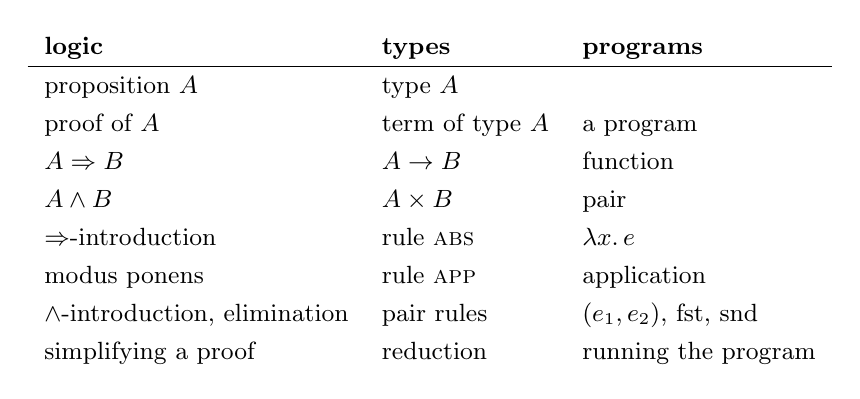
\begin{tikzpicture}[font=\small]
\node[inner sep=0] {\renewcommand{\arraystretch}{1.25}\begin{tabular}{lll}
\textbf{logic} & \textbf{types} & \textbf{programs}\\\hline
proposition $A$ & type $A$ & \\
proof of $A$ & term of type $A$ & a program\\
$A \Rightarrow B$ & $A \to B$ & function\\
$A \wedge B$ & $A \times B$ & pair\\
$\Rightarrow$-introduction & rule \textsc{abs} & $\lambda x.\,e$\\
modus ponens & rule \textsc{app} & application\\
$\wedge$-introduction, elimination & pair rules & $(e_1, e_2)$, \code{fst}, \code{snd}\\
simplifying a proof & reduction & running the program\\
\end{tabular}};
\end{tikzpicture}
\par\smallskip{\small The correspondence, line by line. Read down the middle column, a type is a formula; read down the last, its proofs are the programs of that type.}
\end{omfigure}

The \omterm{def:b3:type-systems:inference}{principal type} of \code{swap} in \cref{out:b3:type-systems:poly}, $\alpha \times \beta \to \beta \times \alpha$, is the tautology $A \wedge B \Rightarrow B \wedge A$, and \code{swap} is its proof. Rust's generics play the same game: a function generic in \code{A} and \code{B} cannot inspect values of those types, so its body can only rearrange what it is given, and a well-typed body that returns is a proof. The proviso matters: a body that loops for ever or calls \code{panic!} has every type, as does a recursive definition that never stops, so a language with general recursion, read as a logic, proves everything. The correspondence holds for the total, terminating fragment.

\omcode{code/bachelor-3/06-type-systems/listings/curry_howard.rs}{1}{23}{Three proofs as generic functions: commutativity of conjunction, modus ponens, and the transitivity of implication.}\label{lst:b3:type-systems:ch}

\omoutput{code/bachelor-3/06-type-systems/outputs/curry_howard.txt}{The proofs run: \code{swap} exchanges, and \code{chain} composes two functions into a third.}\label{out:b3:type-systems:ch}

\begin{recall}
In Rust, assigning a non-\code{Copy} value or passing it by value moves it: the old variable can no longer be used. A borrow lends access without moving (Year 2 volume).
\end{recall}

Types can track more than the shape of a value. Logic itself has systems in which a hypothesis must be used exactly once, and their programs are functions that use each argument once.

\begin{definition}[Linear type, affine type]\label{def:b3:type-systems:linear}
A \emph{linear}\index{linear type} \omterm{def:b3:type-systems:type-system}{type system} requires every variable of certain types to be used exactly once; an \emph{affine}\index{affine type} one, at most once.
\end{definition}

Rust's ownership is \omterm{def:b3:type-systems:linear}{affine}: a value of a type that is not \code{Copy} may be moved once, and a use after the move is a type error, reported before the program runs, exactly as a boolean added to an integer is. The borrow checker extends the idea with borrows, which use a value without consuming it, for a span of the program the checker computes.

\omcode{code/bachelor-3/06-type-systems/listings/borrow_reject.rs}{1}{12}{A vector moved into a function, then used again.}\label{lst:b3:type-systems:borrow}

\omoutput[1-11]{code/bachelor-3/06-type-systems/outputs/borrow_reject.txt}{The compiler's verdict: the use on line~11 needs the value moved on line~10. Like a type error, it names the two places involved.}\label{out:b3:type-systems:borrow}

\begin{inpractice}[Annotate the boundaries]
Inference can type a whole program with no annotation, and the errors then appear far from their cause: a mistake in one function changes its inferred type, and the complaint comes from a caller. Programmers in languages with inference still write the types of top-level and exported functions. The annotation documents the interface, and it stops an error at the function that contains it.
\end{inpractice}

\begin{history}[Principal types]
Roger Hindley published the principal type-scheme of a term of combinatory logic in 1969. % ledger: b3:hindley-1969
Robin Milner published a theory of type polymorphism in programming in 1978. % ledger: b3:milner-1978
In 1982 Luis Damas and Milner published their paper on \omterm{def:b3:type-systems:inference}{principal type} schemes for functional programs. % ledger: b3:damas-milner-1982
The proof of safety by \omterm{def:b3:type-systems:safety}{progress} and \omterm{def:b3:type-systems:safety}{preservation}, as in this chapter, follows a syntactic approach that Andrew Wright and Matthias Felleisen published in 1994. % ledger: b3:wright-felleisen-1994
\end{history}

\section{Exercises}\label{sec:b3:type-systems:exercises}

\begin{exercise}[$\star$]\label{exo:b3:type-systems:1}
Give the type of each term, or say why it has none: \texttt{\textbackslash{}x:\ int.\ \textbackslash{}y:\ bool.\ if y then x else 0}; \texttt{\textbackslash{}f:\ int -> int.\ \textbackslash{}x:\ int.\ f (f x)}; \texttt{(\textbackslash{}x:\ bool.\ x) true}.
\end{exercise}

\begin{exercise}[$\star$]\label{exo:b3:type-systems:2}
Build the \omterm{def:b3:type-systems:judgement}{typing derivation} of \texttt{\textbackslash{}x:\ int.\ \textbackslash{}f:\ int -> bool.\ f x} and count its judgements.
\end{exercise}

\begin{exercise}[$\star$]\label{exo:b3:type-systems:3}
Which of these terms have a type? Give the \omterm{def:b3:type-systems:inference}{principal type} when there is one: \texttt{\textbackslash{}x.\ x x}; \texttt{\textbackslash{}f.\ \textbackslash{}x.\ f x x}; \texttt{\textbackslash{}p.\ fst p + snd p}; \texttt{\textbackslash{}x.\ if x then x else 1}.
\end{exercise}

\begin{exercise}[$\star$]\label{exo:b3:type-systems:4}
Predict the line that \code{infer_demo} would print for \texttt{let twice = \textbackslash{}f.\ \textbackslash{}x.\ f (f x) in \dots{}}.
\end{exercise}

\begin{exercise}[$\star\star$]\label{exo:b3:type-systems:5}
\code{exercises/ex5_noocc.rs} keeps a \emph{triangular} substitution, whose bindings may mention other bound variables, and resolves a type by following them. With \code{occurs_check} false, inferring \texttt{\textbackslash{}x.\ x x} accepts an equation and then never finishes printing the type. Which equation, and why does printing not end? Show that the occurs check fixes it, and explain why it cannot refuse a solvable problem.
\end{exercise}

\begin{exercise}[$\star\star$]\label{exo:b3:type-systems:6}
The checker of \cref{lst:b3:type-systems:check} rejects pairs. Write the rules for $(e_1, e_2)$, \code{fst} and \code{snd}, and a typing function that has them; test it on \texttt{(\textbackslash{}p:\ int * bool.\ if snd p then fst p else 0) (1, true)}.
\end{exercise}

\begin{exercise}[$\star\star$]\label{exo:b3:type-systems:7}
Prove the substitution lemma (\cref{lem:b3:type-systems:substitution}). You will need weakening: a judgement stays true when unused bindings are added to its context.
\end{exercise}

\begin{exercise}[$\star\star$]\label{exo:b3:type-systems:8}
Prove that in the simply typed core, with annotated parameters, a term has at most one type in a given context. Does this hold for the unannotated calculus?
\end{exercise}

\begin{exercise}[$\star\star$]\label{exo:b3:type-systems:9}
Why is \texttt{let id = \textbackslash{}x.\ x in id id} typable, and what is its \omterm{def:b3:type-systems:inference}{principal type}, while \texttt{(\textbackslash{}id.\ id id) (\textbackslash{}x.\ x)} is not?
\end{exercise}

\begin{exercise}[$\star\star\star$]\label{exo:b3:type-systems:10}
Give a \omterm{def:b3:type-systems:judgement}{typing rule} for \texttt{letrec f = \textbackslash{}x.\ e1 in e2} without polymorphism, and prove the case of \omterm{def:b3:type-systems:safety}{preservation} for the step that unfolds it.
\end{exercise}

\begin{exercise}[$\star\star\star$]\label{exo:b3:type-systems:11}
Show that \omterm{def:b3:type-systems:polymorphism}{let-polymorphism} is needed: give a program that \code{Infer} types, and that the same inference with \code{generalise} set to false rejects; explain exactly which equation fails, and say why generalising at \code{let} is sound, given the semantics of \code{let}.
\end{exercise}

\begin{exercise}[$\star\star\star$]\label{exo:b3:type-systems:12}
Add references to the language: \code{ref e} creates a cell, \code{!r} reads it, \code{r := e} writes it, with type $\tau\ \mathtt{ref}$ for a cell holding a $\tau$. Show that generalising \texttt{let r = ref (\textbackslash{}x.\ x) in \dots{}} lets a well-typed program apply a function of type $\mathtt{int} \to \mathtt{int}$ to a boolean. State the \emph{value restriction}, which generalises \code{let x = e} only when $e$ is a value, and explain why it is \omterm{def:b3:type-systems:safety}{safe} and why it still types the programs of \cref{lst:b3:type-systems:poly}.
\end{exercise}

\section{Weekend problem}\label{sec:b3:type-systems:problem}

\begin{problem}[{Weekend problem --- Types that explode}]\label{pb:b3:type-systems:1}
The program \texttt{let f0 = \textbackslash{}x.\ (x, x) in let f1 = \textbackslash{}x.\ f0 (f0 x) in ...\ in fn} defines $n + 1$ functions, each applying the previous one twice. \code{blowup.rs} builds it for $n = 0, \dots, 4$, infers its \omterm{def:b3:type-systems:inference}{principal type} $\text{\ttfamily\textquotesingle a} \to T_n$, and measures $T_n$ two ways: as a tree, by its leaves, and as a graph in which equal subtrees are drawn once.

\omoutput{code/bachelor-3/06-type-systems/outputs/blowup.txt}{For each $n$: the program's length in characters, the calls to \code{unify}, the leaves of $T_n$, and its distinct subtrees.}\label{out:b3:type-systems:blowup}

\needspace{4\baselineskip}\medskip\noindent\textbf{Part I --- By hand.}
\begin{enumerate}
\item Infer the \omterm{def:b3:type-systems:inference}{principal type} of \texttt{\textbackslash{}x.\ (x, x)}, writing every equation.
\item Infer the type of \texttt{let f0 = \textbackslash{}x.\ (x, x) in \textbackslash{}x.\ f0 (f0 x)}. Where are the two instances of $f_0$'s scheme used?
\item What is the type of \code{f0 (f0 1)}?
\item Why is \texttt{(\textbackslash{}f0.\ \textbackslash{}x.\ f0 (f0 x)) (\textbackslash{}x.\ (x, x))} rejected? Write the equation that fails.
\item Write $T_1$ and $T_2$.
\item How does the program's length grow with $n$?
\end{enumerate}

\needspace{4\baselineskip}\medskip\noindent\textbf{Part II --- The family.}
\begin{enumerate}[resume]
\item Show that $T_k = T_{k-1}[\text{\ttfamily\textquotesingle a} := T_{k-1}]$ for $k \ge 1$, with $T_0 = \text{\ttfamily\textquotesingle a} \times \text{\ttfamily\textquotesingle a}$.
\item Deduce the number of leaves $\ell_k$ of $T_k$: give a recurrence, then a closed form.
\item Give the depth of $T_k$.
\item Count the distinct subtrees of $T_k$, and explain the column of \cref{out:b3:type-systems:blowup}.
\item Check the three formulas against the table.
\item What would the row $n = 5$ say? Why does the program not print it?
\end{enumerate}

\needspace{4\baselineskip}\medskip\noindent\textbf{Part III --- Where the time goes.}
\begin{enumerate}[resume]
\item The unify calls grow by 6 per line. Which equations does each \code{let} line contribute?
\item If unification is called so few times, where does the work of inference go when types are trees?
\item Estimate the memory for $T_5$ as a tree, at 16 bytes per node.
\item With types as graphs (each subtree shared), what is the size of $T_n$? Is inference then polynomial in the program's length?
\item Printing $T_n$ costs its number of leaves at least. What does this say of any algorithm that outputs \omterm{def:b3:type-systems:inference}{principal types} as text?
\item Harry Mairson showed in 1990 that deciding whether an ML program has a type is complete for deterministic exponential time. % ledger: b3:mairson-1990
What does this add to the observation of the previous question?
\end{enumerate}

\needspace{4\baselineskip}\medskip\noindent\textbf{Part IV --- Why it does not happen.}
\begin{enumerate}[resume]
\item Which feature of the family produces the growth: the pairs, the nesting of \code{let}, or the doubling? Remove each in turn and say what remains.
\item Real programs nest \code{let}s deeply. Why do their types stay small?
\item What does a type annotation on \code{f1} change for the checker's work?
\item Would the explosion happen in the simply typed core, where each parameter carries its type? Where would the size go?
\item What does a compiler with inference do to keep its error messages readable when a type is large?
\item Sum up: give the size of $T_n$ as a tree and as a graph, and the cost of inference on this family in terms of the program's length.
\end{enumerate}
\end{problem}
